% ============================================================
%  Lecture Script: Polynomial ALSSM Basis Classes in lmlib
%  AlssmPoly | AlssmPolyJordan | AlssmPolyLegendre | AlssmPolyMeixner
% ============================================================
\documentclass[11pt, a4paper]{article}

\usepackage{amsmath, amssymb, amsthm}
\usepackage{mathtools}   % provides \coloneqq
\usepackage{bm}
\usepackage{booktabs}
\usepackage{geometry}
\usepackage{hyperref}
\usepackage{xcolor}
\usepackage{tikz}
\usepackage{pgfplots}
\pgfplotsset{compat=1.18}
\usetikzlibrary{patterns}

\geometry{left=2.5cm, right=2.5cm, top=2.5cm, bottom=2.5cm}

\theoremstyle{definition}
\newtheorem{definition}{Definition}
\newtheorem{proposition}{Proposition}
\newtheorem{remark}{Remark}

\newcommand{\R}{\mathbb{R}}
\newcommand{\N}{\mathbb{N}}
\newcommand{\vx}{\bm{x}}
\newcommand{\vC}{\bm{C}}
\newcommand{\mA}{\bm{A}}
\newcommand{\mphi}{\bm{\phi}}
\newcommand{\haty}{\hat{y}}
\newcommand{\defeq}{\coloneqq}
\newcommand{\triu}{\operatorname{triu}}

\title{\textbf{Polynomial Basis Classes for ALSSMs}\\[0.5em]
\large A Lecture on \texttt{AlssmPoly}, \texttt{AlssmPolyJordan},\\
\texttt{AlssmPolyLegendre}, and \texttt{AlssmPolyMeixner}}
\author{lmlib Internals Lecture Series}
\date{}

\begin{document}
\maketitle
\tableofcontents
\bigskip

% ============================================================
\section{Background: The ALSSM Signal Model}
% ============================================================

An \emph{autonomous linear state-space model} (ALSSM) represents a signal
trajectory as
\begin{equation}
  s_j(\vx) \defeq \vC \mA^j \vx, \qquad j = 0, 1, 2, \ldots
  \label{eq:alssm}
\end{equation}
where $\mA \in \R^{N \times N}$ is the \emph{state-transition matrix},
$\vC \in \R^{1 \times N}$ is the \emph{output vector}, and
$\vx \in \R^N$ is the \emph{state vector} holding the model parameters
\cite{Wildhaber2019, Zalmai2017}.

The lag index $j$ increases into the past: $j=0$ is the current sample,
$j=1$ the previous one, etc.  The signal model at each time step $k$ is
therefore
\[
  y[k-j] \approx s_j(\vx[k]) = \vC \mA^j \vx[k].
\]

\medskip
\noindent\textbf{The key design freedom.}
For polynomial signal models, the choice of $\mA$ and $\vC$ is not unique:
many $(\mA, \vC)$ pairs represent the same family of degree-$D$ polynomials,
but they differ dramatically in their numerical properties (Gram-matrix
conditioning, recursion stability, and parameter interpretability).  The four
classes discussed in this lecture each make a different and well-motivated
choice, summarised in Table~\ref{tab:summary}.

\begin{table}[h]
\centering
\caption{Summary of the four polynomial ALSSM classes.}
\label{tab:summary}
\renewcommand{\arraystretch}{1.3}
\begin{tabular}{lllll}
\toprule
Class & Basis $\mphi(j)$ & $\mA$ structure & $\vC$ & Window \\
\midrule
\texttt{AlssmPoly}         & Monomials $j^n$             & Upper Pascal        & $[1,0,\ldots]$                   & any \\
\texttt{AlssmPolyJordan}   & Falling factorials $\binom{j}{n}$ & Jordan block   & $[1,0,\ldots]$                   & any \\
\texttt{AlssmPolyLegendre} & Legendre $P_n(t_j)$         & Legendre shift      & $[P_n(-1)]$                      & finite \\
\texttt{AlssmPolyMeixner}  & Meixner $M_n(j;\gamma)$     & Near-identity       & $[1,1,\ldots,1]$                 & $\infty$ \\
\bottomrule
\end{tabular}
\end{table}

% ============================================================
\section{The Central Design Principle: Shift Consistency}
% ============================================================

All four classes share one structural requirement that turns~\eqref{eq:alssm}
into a \emph{recursively computable} filter.  Define the \emph{design-matrix
row} at lag $j$ as the row vector
\[
  \mphi(j) \defeq \vC \mA^j \in \R^{1 \times N}.
\]
For polynomial models we want $\mphi(j) = [\phi_0(j),\, \phi_1(j),\, \ldots,\,
\phi_D(j)]$ where $\{\phi_n\}$ are the chosen basis polynomials.  The
ALSSM recursion $\vx[k] = \mA\,\vx[k-1]$ is valid \emph{only if} the basis
satisfies the \textbf{shift consistency property}:
\begin{equation}
  \mphi(j+1) = \mphi(j)\,\mA, \quad \forall j \geq 0.
  \label{eq:shift}
\end{equation}
Equation~\eqref{eq:shift} imposes that $\mA$ is the matrix representation
of the operator ``evaluate the basis one step further into the past''.
Equivalently, column $n$ of $\mA$ contains the coefficients of $\phi_n(j+1)$
expanded in the basis $\{\phi_k(j)\}$:
\[
  \phi_n(j+1) = \sum_{k=0}^{D} A_{kn}\,\phi_k(j).
\]
Each of the four classes derives $\mA$ by enforcing this identity for a
specific polynomial family.  The derivations follow in Sections~\ref{sec:poly}
through~\ref{sec:meixner}.

% ============================================================
\section{\texttt{AlssmPoly}: Monomial (Pascal) Basis}
\label{sec:poly}
% ============================================================

\subsection{The polynomial family}

The simplest choice is the monomial basis $\phi_n(j) = j^n$, giving the
general degree-$D$ polynomial
\begin{equation}
  s_j(\vx) = \sum_{n=0}^{D} x_n\, j^n
           = x_0 + x_1 j + x_2 j^2 + \cdots + x_D j^D.
\end{equation}
The state vector $\vx = [x_0, x_1, \ldots, x_D]^\top$ holds the
standard polynomial coefficients directly.

\subsection{Degree-2 example}

For $D=2$ the model is $s_j = x_0 + x_1 j + x_2 j^2$.  With
$\vx = [2,\,-1,\,0.5]^\top$ (i.e.\ $s_j = 2 - j + 0.5 j^2$) the
trajectory reads $s_0=2,\; s_1=1.5,\; s_2=2,\; s_3=3.5,\;\ldots$

\begin{center}
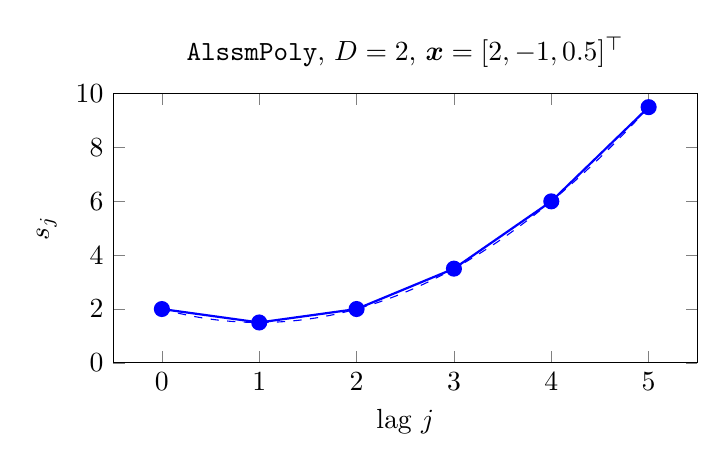
\begin{tikzpicture}
\begin{axis}[
  xlabel={lag $j$}, ylabel={$s_j$},
  title={\texttt{AlssmPoly}, $D=2$, $\vx=[2,-1,0.5]^\top$},
  xtick={0,1,2,3,4,5}, width=9cm, height=5cm,
  ymin=0, ymax=10,
  mark size=2.5pt
]
\addplot[blue, thick, mark=*, mark options={fill=blue}]
  coordinates {(0,2)(1,1.5)(2,2)(3,3.5)(4,6)(5,9.5)};
\addplot[blue, dashed, domain=0:5, samples=80]
  {2 - x + 0.5*x^2};
\end{axis}
\end{tikzpicture}
\end{center}

\subsection{State-transition matrix and output vector}

\begin{equation}
  \mA = \begin{bmatrix}
    1 & 1 & 1 \\
    0 & 1 & 2 \\
    0 & 0 & 1
  \end{bmatrix},
  \qquad
  \vC = [1,\; 0,\; 0].
\end{equation}
The $n$-th column of $\mA$ contains the binomial coefficients
$\binom{n}{k}$ for $k = 0, 1, \ldots, n$, so $\mA$ is the \emph{upper
Pascal matrix} of order $N = D+1$.

\subsection{Derivation of \texorpdfstring{$\mA$}{A}}

We must find $\mA$ such that $\mphi(j+1) = \mphi(j)\,\mA$ where
$\mphi(j) = [1,\, j,\, j^2,\, \ldots,\, j^D]$.  Column $n$ of $\mA$
must express $\phi_n(j+1) = (j+1)^n$ in terms of the basis evaluated
at $j$.  By the \textbf{binomial theorem}:
\begin{equation}
  (j+1)^n = \sum_{k=0}^{n} \binom{n}{k} j^k.
  \label{eq:binomial}
\end{equation}
Comparing with $\phi_n(j+1) = \sum_k A_{kn}\,\phi_k(j) = \sum_k A_{kn}\,
j^k$, we read off
\[
  A_{kn} = \binom{n}{k}, \quad 0 \leq k \leq n; \qquad A_{kn} = 0 \text{ for }
  k > n.
\]
This is precisely the \emph{upper Pascal matrix}.

\medskip
\noindent\textbf{Worked example for $D=2$.}
Expanding the three columns explicitly:
\begin{align*}
  n=0: &\quad (j+1)^0 = 1 = \binom{0}{0}\cdot j^0 \\
       &\quad \Rightarrow A_{00}=1, \text{ all other } A_{k0}=0.\\[4pt]
  n=1: &\quad (j+1)^1 = j + 1 = \binom{1}{0}\cdot j^0 + \binom{1}{1}\cdot j^1 \\
       &\quad \Rightarrow A_{01}=1,\; A_{11}=1.\\[4pt]
  n=2: &\quad (j+1)^2 = j^2 + 2j + 1
               = \binom{2}{0}\cdot j^0 + \binom{2}{1}\cdot j^1 + \binom{2}{2}\cdot j^2 \\
       &\quad \Rightarrow A_{02}=1,\; A_{12}=2,\; A_{22}=1.
\end{align*}
Reading off the binomial coefficients column by column:
\[
  \mA = \begin{bmatrix}
    \binom{0}{0} & \binom{1}{0} & \binom{2}{0} \\
    0            & \binom{1}{1} & \binom{2}{1} \\
    0            & 0            & \binom{2}{2}
  \end{bmatrix}
  =
  \begin{bmatrix}
    1 & 1 & 1 \\
    0 & 1 & 2 \\
    0 & 0 & 1
  \end{bmatrix}.
\]
For completeness, the general form for any degree $D$:
\[
  \mA = \begin{bmatrix}
    1 & 1 & 1 & 1 & \cdots \\
    0 & 1 & 2 & 3 & \cdots \\
    0 & 0 & 1 & 3 & \cdots \\
    0 & 0 & 0 & 1 & \cdots \\
    \vdots & & & & \ddots
  \end{bmatrix}.
\]
The output vector $\vC = [1, 0, \ldots, 0]$ evaluates $s_0 = x_0$,
which is the polynomial value at the current sample ($j=0$).  This
follows from $\vC \mA^0 \vx = \vC \vx = x_0 = \vx|_{j=0}$.

\begin{remark}
The Pascal matrix is generated in lmlib via \texttt{scipy.linalg.pascal(N, kind='upper')}.
Its entries grow exponentially with degree and window size, causing the Gram
matrix $W = \sum_j \gamma^j \mphi(j)^\top \mphi(j)$ to have condition
number $\kappa(W) = \mathcal{O}(g^{2D})$ for effective window size $g$.
This is the main motivation for the alternative bases in the following
sections.
\end{remark}

% ============================================================
\section{\texttt{AlssmPolyJordan}: Falling-Factorial (Jordan) Basis}
\label{sec:jordan}
% ============================================================

\subsection{The polynomial family}

The Jordan basis replaces monomials $j^n$ with \emph{falling factorial}
polynomials (also called \emph{binomial coefficients in $j$}):
\begin{equation}
  \phi_n(j) \defeq \binom{j}{n} = \frac{j!}{n!\,(j-n)!}
           = \frac{j(j-1)\cdots(j-n+1)}{n!}, \quad
  \phi_0(j) = 1.
\end{equation}
The signal model is
\begin{equation}
  s_j(\vx) = \sum_{n=0}^{D} x_n \binom{j}{n}
           = x_0 + x_1 j + x_2 \frac{j(j-1)}{2} + \cdots
\end{equation}
Since $\binom{j}{n}$ is a degree-$n$ polynomial in $j$, this spans the
same function space as \texttt{AlssmPoly}.  The state coefficients
$x_n$ are the \emph{Newton forward-difference coefficients} of the signal
rather than the standard polynomial coefficients \cite{Zalmai2017}.

\subsection{Degree-2 example}

For $D=2$ the model is $s_j = x_0 + x_1 j + x_2 j(j-1)/2$.  With
$\vx = [2,\,-1,\,1]^\top$:
\begin{center}
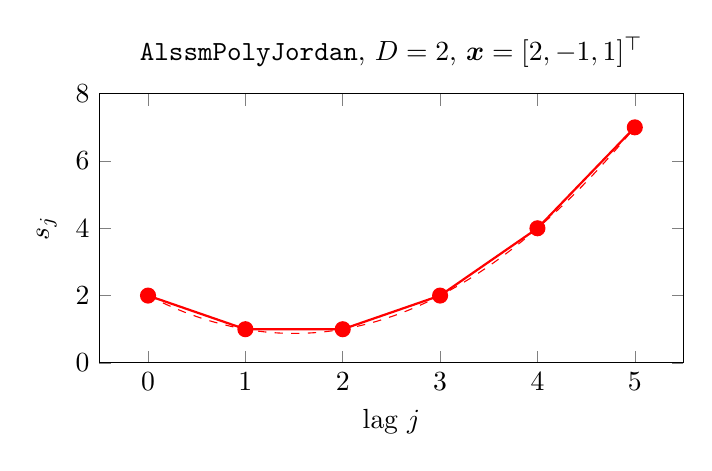
\begin{tikzpicture}
\begin{axis}[
  xlabel={lag $j$}, ylabel={$s_j$},
  title={\texttt{AlssmPolyJordan}, $D=2$, $\vx=[2,-1,1]^\top$},
  xtick={0,1,2,3,4,5}, width=9cm, height=5cm,
  ymin=0, ymax=8,
  mark size=2.5pt
]
\addplot[red, thick, mark=*, mark options={fill=red}]
  coordinates {(0,2)(1,1)(2,1)(3,2)(4,4)(5,7)};
\addplot[red, dashed, domain=0:5, samples=80]
  {2 - x + x*(x-1)/2};
\end{axis}
\end{tikzpicture}
\end{center}

\subsection{State-transition matrix and output vector}

\begin{equation}
  \mA = \begin{bmatrix}
    1 & 1 & 0 \\
    0 & 1 & 1 \\
    0 & 0 & 1
  \end{bmatrix},
  \qquad
  \vC = [1,\; 0,\; 0].
\end{equation}
This is the \emph{Jordan block} for eigenvalue $1$: the identity matrix
plus a superdiagonal of ones.  It is called the Jordan normal form because
it represents the nilpotent shift operator acting on a chain of generalised
eigenvectors \cite{Horn1985}.

\subsection{Derivation of \texorpdfstring{$\mA$}{A}}

We must verify that $\mphi(j+1) = \mphi(j)\,\mA$ with
$\mphi(j) = \bigl[\binom{j}{0}, \binom{j}{1}, \binom{j}{2}, \ldots\bigr]$.
This follows directly from \textbf{Pascal's identity}:
\begin{equation}
  \binom{j+1}{n} = \binom{j}{n} + \binom{j}{n-1}.
  \label{eq:pascal}
\end{equation}
Identifying $A_{kn}$ such that $\phi_n(j+1) = \sum_k A_{kn}\phi_k(j)$:
\[
  \binom{j+1}{n} = \binom{j}{n} + \binom{j}{n-1}
  \;\Longrightarrow\;
  A_{nn} = 1, \quad A_{n-1,n} = 1, \quad A_{kn} = 0 \text{ otherwise}.
\]
This gives the Jordan block $\mA = I + \mathrm{superdiag}(\mathbf{1})$.
The formula $A_{kn} = \delta_{k,n} + \delta_{k,n-1}$ creates the two
diagonals directly, without any free parameters.

\begin{remark}[Comparison with \texttt{AlssmPoly}]
Both bases span the same polynomial space. The Jordan basis has a far
simpler $\mA$ (bidiagonal vs.\ full upper triangular), and its condition
number $\kappa(\mA)$ grows more slowly with degree. However, both still
suffer from ill-conditioned Gram matrices for large windows, because the
design-matrix rows $\mphi(j)$ grow with $j$ in both bases. The Legendre
and Meixner bases address this directly.
\end{remark}

% ============================================================
\section{\texttt{AlssmPolyLegendre}: Legendre Basis on a Finite Window}
\label{sec:legendre}
% ============================================================

\subsection{Motivation}

For a finite window $[0, W]$, the monomial and falling-factorial design
matrices become ill-conditioned because $\phi_n(j) = j^n$ or
$\binom{j}{n}$ grow with $j$. The classical remedy is to \emph{normalise}
the lag index to a fixed interval and use an orthogonal polynomial basis.

\subsection{The polynomial family}

Let $W = b - a$ be the window width. Define the \emph{scaled lag}
\begin{equation}
  t_j \defeq \frac{2j}{W} - 1 \in [-1,+1], \qquad j \in [0, W],
  \label{eq:tsc}
\end{equation}
with step size $h = 2/W$.  The basis functions are the \emph{Legendre
polynomials} $P_n(t)$, which satisfy the three-term recurrence
\begin{equation}
  (n+1)P_{n+1}(t) = (2n+1)\,t\,P_n(t) - n\,P_{n-1}(t),
  \quad P_0(t)=1,\; P_1(t)=t.
  \label{eq:legendre3term}
\end{equation}
The signal model is
\begin{equation}
  s_j(\vx) = \sum_{n=0}^{D} x_n\, P_n(t_j).
\end{equation}
Key property: $\{P_n\}$ are orthogonal under the $L^2[-1,1]$ inner product,
\[
  \int_{-1}^{1} P_m(t)\,P_n(t)\,dt = \frac{2}{2n+1}\,\delta_{mn},
\]
where $\delta_{mn}$ is the \emph{Kronecker delta} ($\delta_{mn}=1$ if $m=n$,
$\delta_{mn}=0$ otherwise): the integral is zero whenever $m \neq n$
(orthogonality) and equals $2/(2n+1)$ when $m=n$ (the squared norm).
This makes the continuous Gram matrix perfectly diagonal
\cite{Abramowitz1972, DLMF}.

\subsection{Degree-2 example ($W=10$, $h=0.2$)}

With $D=2$, $a_\text{seg}=0$, $b_\text{seg}=10$ the state
$\vx = [1,\, 0,\, 0]^\top$ gives the constant function $s_j = P_0(t_j) = 1$;
state $\vx = [0,\, 1,\, 0]^\top$ gives the ramp $s_j = t_j = h j - 1$; and
$\vx = [0,\, 0,\, 1]^\top$ gives the parabola $s_j = P_2(t_j) = (3t_j^2-1)/2$.

\begin{center}
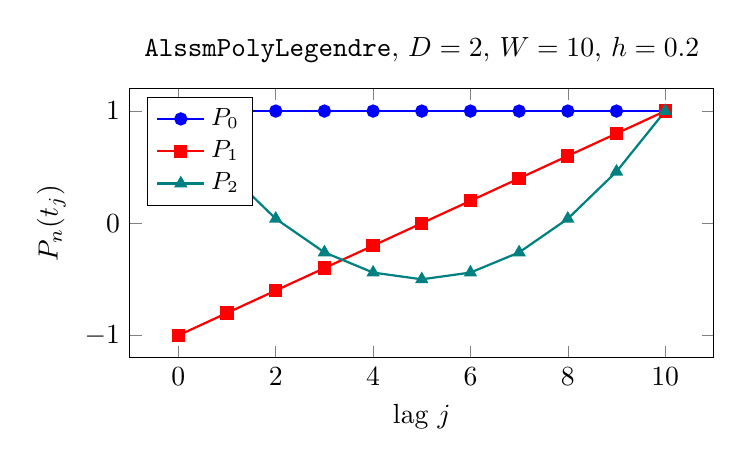
\begin{tikzpicture}
\begin{axis}[
  xlabel={lag $j$}, ylabel={$P_n(t_j)$},
  title={\texttt{AlssmPolyLegendre}, $D=2$, $W=10$, $h=0.2$},
  xtick={0,2,4,6,8,10},
  width=9cm, height=5cm,
  legend pos=north west,
  legend style={font=\small},
  mark size=2pt
]
\addplot[blue, thick, mark=*, mark options={fill=blue}]
  coordinates {(0,1)(1,1)(2,1)(3,1)(4,1)(5,1)(6,1)(7,1)(8,1)(9,1)(10,1)};
\addlegendentry{$P_0$}
\addplot[red, thick, mark=square*, mark options={fill=red}]
  coordinates {(0,-1)(1,-0.8)(2,-0.6)(3,-0.4)(4,-0.2)(5,0)(6,0.2)(7,0.4)(8,0.6)(9,0.8)(10,1)};
\addlegendentry{$P_1$}
\addplot[teal, thick, mark=triangle*, mark options={fill=teal}]
  coordinates {(0,1)(1,0.46)(2,0.04)(3,-0.26)(4,-0.44)(5,-0.5)(6,-0.44)(7,-0.26)(8,0.04)(9,0.46)(10,1)};
\addlegendentry{$P_2$}
\end{axis}
\end{tikzpicture}
\end{center}

\subsection{State-transition matrix and output vector}

For $D=2$, $W=10$ (i.e.\ $h=1/5$):
\begin{equation}
  \mA = \begin{bmatrix}
    1 & h & \tfrac{3}{2}h^2 \\[2pt]
    0 & 1 & 3h \\
    0 & 0 & 1
  \end{bmatrix}
  =
  \begin{bmatrix}
    1 & 0.2 & 0.06 \\
    0 & 1   & 0.6  \\
    0 & 0   & 1
  \end{bmatrix},
  \qquad
  \vC = \bigl[P_0(-1),\; P_1(-1),\; P_2(-1)\bigr] = [1,\; -1,\; 1].
\end{equation}
The matrix $\mA$ is upper-triangular with unit diagonal and is called the
\emph{Legendre shift matrix}; it has condition number $\kappa(\mA) \approx 1$
independently of $W$.

\subsection{Derivation of \texorpdfstring{$\mA$}{A}: Taylor shift in the Legendre basis}

The shift $j \to j+1$ corresponds to $t \to t + h$ in the scaled
coordinate.  We must express $P_n(t+h)$ as a linear combination of
$P_0(t), \ldots, P_n(t)$, i.e.\ find the column $n$ of $\mA$.

Expanding via the \textbf{Taylor series}:
\begin{equation}
  P_n(t+h) = \sum_{m=0}^{n} \frac{h^m}{m!}\, P_n^{(m)}(t),
  \label{eq:taylor}
\end{equation}
where $P_n^{(m)}$ is the $m$-th derivative.  Since $P_n^{(m)}$ is a
polynomial of degree $n-m$, it can be expanded in the Legendre basis:
\[
  P_n^{(m)}(t) = \sum_{k=0}^{n-m} \bigl[\mathbf{D}^m e_n\bigr]_k P_k(t),
\]
where $\mathbf{D}$ is the differentiation operator in Legendre coefficient
space (implemented by \texttt{numpy.polynomial.legendre.legder}), and
$e_n$ is the unit vector with a $1$ in position $n$.  Substituting:
\begin{equation}
  P_n(t+h) = \sum_{m=0}^{n} \frac{h^m}{m!}
             \sum_{k=0}^{n-m} \bigl[\mathbf{D}^m e_n\bigr]_k P_k(t).
\end{equation}
The coefficient of $P_k(t)$ in $P_n(t+h)$ is
\[
  A_{kn} = \sum_{m=0}^{n-k} \frac{h^m}{m!} \bigl[\mathbf{D}^m e_n\bigr]_k.
\]
This formula is \emph{exact} (not an approximation) because the Taylor
series of a polynomial terminates after finitely many terms.  It
requires only $O(N^2)$ operations and produces column $n$ of $\mA$
without any matrix inversion.

For $D=2$, $h=1/5$, the three columns work out as follows.
\begin{itemize}
  \item $n=0$: $P_0(t+h) = 1 = P_0(t)$, so column 0 = $[1,0,0]^\top$.
  \item $n=1$: $P_1(t+h) = t+h = P_1(t) + h\,P_0(t)$, so column 1 = $[h,1,0]^\top = [0.2,1,0]^\top$.
  \item $n=2$: $P_2(t+h) = \tfrac{3}{2}(t+h)^2 - \tfrac{1}{2}$
    $= \tfrac{3}{2}t^2 + 3th + \tfrac{3}{2}h^2 - \tfrac{1}{2}$
    $= P_2(t) + 3h\,P_1(t) + \tfrac{3}{2}h^2\,P_0(t)$;
    with $h=1/5$: column 2 = $[\tfrac{3}{2}\cdot\tfrac{1}{25},\;3\cdot\tfrac{1}{5},\;1]^\top = [0.06,\;0.6,\;1]^\top$.
\end{itemize}
This exactly matches the numerical $\mA$ above.

\begin{remark}[Output vector $\vC$]
The output vector evaluates the polynomial at the \emph{current} sample,
which has lag $j=0$ and thus scaled coordinate $t_0 = -1$.  Since
$P_n(-1) = (-1)^n$, the output vector is the alternating-sign vector
$\vC = [1, -1, 1, -1, \ldots]$.  When the segment window starts at
$a_\text{seg} \neq 0$, lmlib applies the additional shift
$\vC \leftarrow \vC\, \mA^{-a_\text{seg}}$ to keep the evaluation at
$j=0$.
\end{remark}

\begin{remark}[Gram-matrix conditioning]
The Gram matrix $W_{\rm ss} = V^\top \operatorname{diag}(\gamma^j) V$,
where $V_{jn} = P_n(t_j)$, has condition number
$\kappa(W_{\rm ss}) \approx 2D+1$ for all practical window sizes.
This is a reduction from $\kappa = \mathcal{O}(W^{2D})$
for the monomial basis.  The Legendre Vandermonde formula
$W_{\rm ss} = V^\top \operatorname{diag}(w)\,V$ is computed directly
without solving any linear system, giving exact results for any degree.
\end{remark}

% ============================================================
\section{\texttt{AlssmPolyMeixner}: Meixner Basis on a Semi-Infinite Window}
\label{sec:meixner}
% ============================================================

\subsection{Motivation}

\texttt{AlssmPolyLegendre} requires the window to be finite.  For
infinite or semi-infinite windows (as in the two-sided filter of
\texttt{ex122.0} or the baseline segments of \texttt{ex111.0}),
the window length is not a fixed integer but is controlled by the
exponential decay rate $\gamma = (g-1)/g$.  A basis that is
\emph{orthogonal under the geometric weight $\gamma^j$} on
$j = 0, 1, 2, \ldots$ is needed.

\subsection{The Meixner polynomial family}

The \textbf{Meixner polynomials} $M_n(j;\, 1,\, \gamma)$ are a family
of \emph{discrete orthogonal polynomials}: they are polynomials in the
integer variable $j \in \{0, 1, 2, \ldots\}$, as opposed to the Legendre
polynomials which are defined on a continuous interval. They satisfy the
discrete orthogonality relation
\begin{equation}
  \sum_{j=0}^{\infty} \gamma^j\, M_m(j)\, M_n(j)
  = \frac{\delta_{mn}}{(1-\gamma)\,\gamma^n},
  \label{eq:meixner_orthog}
\end{equation}
for all $m, n \geq 0$, where $0 < \gamma < 1$ \cite{Koekoek1998}.

\paragraph{Reading equation~\eqref{eq:meixner_orthog}.}
This relation expresses two things at once via the Kronecker delta $\delta_{mn}$:
\begin{itemize}
  \item \textbf{Orthogonality} ($m \neq n$): the sum on the left is zero,
    meaning different basis polynomials are uncorrelated under the
    geometric weight.
  \item \textbf{Non-unit norm} ($m = n$): the sum equals
    $1/[(1-\gamma)\gamma^n] = g\cdot(g/(g-1))^n > 0$, which grows
    with degree $n$.  The polynomials are orthogonal but \emph{not}
    orthonormal; they are normalised such that $M_n(0;\,1,\gamma) = 1$
    (see~\eqref{eq:meixner_at_zero} below), not to unit $\ell^2$ norm.
\end{itemize}
That the diagonal entries are not zero is therefore correct and expected:
they represent the squared norms $\|M_n\|^2_{\gamma}$ of the basis
polynomials under the geometric inner product.

\medskip
The Meixner polynomials are given explicitly by the hypergeometric series
\begin{equation}
  M_n(j;\, 1,\, \gamma) = {}_2F_1\!\left(-n,\, -j;\, 1;\, 1-\tfrac{1}{\gamma}\right)
  = \sum_{k=0}^{\min(n,j)} (-1)^k \binom{n}{k}\binom{j}{k}\left(1-\tfrac{1}{\gamma}\right)^{\!k},
  \label{eq:meixner_explicit}
\end{equation}
where ${}_2F_1$ is the Gauss hypergeometric function.

Two special values are essential:
\begin{align}
  M_n(0;\, 1,\, \gamma) &= 1 \quad\text{for all }n \geq 0,
    \label{eq:meixner_at_zero}\\[4pt]
  \sum_{j=0}^{\infty} \gamma^j\,\bigl[M_n(j;\,1,\gamma)\bigr]^2
    &= \frac{1}{(1-\gamma)\,\gamma^n} \quad\text{for all }n \geq 0.
    \label{eq:meixner_norm}
\end{align}
Equation~\eqref{eq:meixner_at_zero} follows because setting $j=0$ kills every
term in~\eqref{eq:meixner_explicit} except $k=0$, giving
$(-1)^0\binom{n}{0}\binom{0}{0}(1-1/\gamma)^0=1$.
Equation~\eqref{eq:meixner_norm} is the squared $\ell^2_\gamma$-norm of $M_n$:
it equals the diagonal entry $W_{\rm ss}[n,n]$ of the steady-state Gram
matrix, and follows from~\eqref{eq:meixner_orthog} with $m=n$.

\subsection{Degree-2 example ($g=5$, $\gamma=4/5$)}

The first three Meixner polynomials for $\gamma = 4/5$ evaluate as
$M_0(j) = 1$, $M_1(j) = 1 - j/4$, and $M_2(j)$ as given in the table
below ($1-1/\gamma = -1/4$):

\begin{center}
\begin{tabular}{cccc}
\toprule
$j$ & $M_0(j)$ & $M_1(j)$ & $M_2(j)$ \\
\midrule
0 & 1 & 1 & 1 \\
1 & 1 & 0.750 & 0.500 \\
2 & 1 & 0.500 & 0.063 \\
3 & 1 & 0.250 & $-$0.313 \\
4 & 1 & 0 & $-$0.625 \\
5 & 1 & $-$0.250 & $-$0.875 \\
\bottomrule
\end{tabular}
\end{center}

\begin{center}
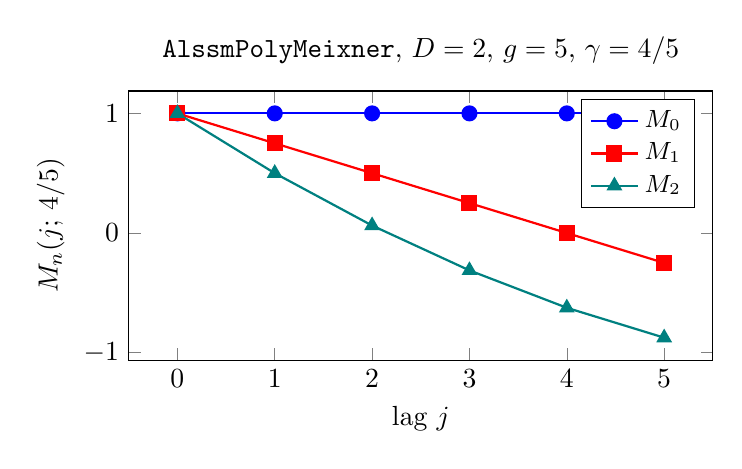
\begin{tikzpicture}
\begin{axis}[
  xlabel={lag $j$}, ylabel={$M_n(j;\,4/5)$},
  title={\texttt{AlssmPolyMeixner}, $D=2$, $g=5$, $\gamma=4/5$},
  xtick={0,1,2,3,4,5},
  width=9cm, height=5cm,
  legend pos=north east,
  legend style={font=\small},
  mark size=2.5pt
]
\addplot[blue, thick, mark=*, mark options={fill=blue}]
  coordinates {(0,1)(1,1)(2,1)(3,1)(4,1)(5,1)};
\addlegendentry{$M_0$}
\addplot[red, thick, mark=square*, mark options={fill=red}]
  coordinates {(0,1)(1,0.75)(2,0.5)(3,0.25)(4,0)(5,-0.25)};
\addlegendentry{$M_1$}
\addplot[teal, thick, mark=triangle*, mark options={fill=teal}]
  coordinates {(0,1)(1,0.5)(2,0.0625)(3,-0.3125)(4,-0.625)(5,-0.875)};
\addlegendentry{$M_2$}
\end{axis}
\end{tikzpicture}
\end{center}

\subsection{State-transition matrix and output vector}

For general $g$ (and $\gamma = (g-1)/g$, $D \geq 1$):
\begin{equation}
  \mA = I_N - \frac{1}{g-1}\,\triu(\mathbf{1}_N,\, 1)
  =
  \begin{bmatrix}
    1 & -\tfrac{1}{g-1} & -\tfrac{1}{g-1} & \cdots \\
    0 & 1               & -\tfrac{1}{g-1} & \cdots \\
    0 & 0               & 1               & \cdots \\
    \vdots & & & \ddots
  \end{bmatrix},
  \qquad
  \vC = [1,\; 1,\; \ldots,\; 1].
  \label{eq:meixner_A}
\end{equation}
For $g=5$ ($\gamma=4/5$), $D=2$:
\begin{equation}
  \mA = \begin{bmatrix}
    1 & -0.25 & -0.25 \\
    0 & 1     & -0.25 \\
    0 & 0     & 1
  \end{bmatrix}, \qquad \vC = [1,\; 1,\; 1].
\end{equation}
The output vector $\vC = \mathbf{1}^\top$ follows from~\eqref{eq:meixner_at_zero}:
evaluating at $j=0$ gives $s_0 = \sum_n x_n M_n(0) = \sum_n x_n$.

\subsection{Derivation of \texorpdfstring{$\mA$}{A}}

We must find $\mA$ such that
$\mphi(j+1) = \mphi(j)\,\mA$ where $\mphi(j) = [M_0(j), M_1(j), \ldots, M_D(j)]$.
Column $n$ of $\mA$ must express $M_n(j+1)$ as a linear combination of
$M_0(j), \ldots, M_D(j)$.

\medskip
\noindent\textbf{Step 1: Forward difference from the explicit formula.}
Starting from~\eqref{eq:meixner_explicit} we compute the first-order
forward difference $\Delta[M_n](j) \defeq M_n(j+1) - M_n(j)$:
\[
  \Delta[M_n](j)
  = \sum_{k=0}^{n} (-1)^k\binom{n}{k}\!\left(1-\tfrac{1}{\gamma}\right)^k
    \!\bigl[\binom{j+1}{k} - \binom{j}{k}\bigr].
\]
By \textbf{Pascal's identity} $\binom{j+1}{k} - \binom{j}{k} = \binom{j}{k-1}$,
so the $k=0$ term vanishes and we shift $k \to k+1$:
\begin{equation}
  \Delta[M_n](j)
  = -\!\left(1-\tfrac{1}{\gamma}\right)\!
    \sum_{k=0}^{n-1} (-1)^k\binom{n}{k+1}\!\left(1-\tfrac{1}{\gamma}\right)^k
    \binom{j}{k}.
  \label{eq:diff1}
\end{equation}

\medskip
\noindent\textbf{Step 2: Express as a partial sum of Meixner polynomials.}
From~\eqref{eq:meixner_explicit}, summing over $m = 0, 1, \ldots, n-1$:
\[
  \sum_{m=0}^{n-1} M_m(j)
  = \sum_{k=0}^{n-1} (-1)^k\!\left(1-\tfrac{1}{\gamma}\right)^k\binom{j}{k}
    \underbrace{\sum_{m=k}^{n-1}\binom{m}{k}}_{= \binom{n}{k+1}},
\]
where the inner sum is evaluated by the \textbf{hockey-stick identity}
\cite{Graham1994}:
\begin{equation}
  \sum_{m=k}^{n-1}\binom{m}{k} = \binom{n}{k+1}.
  \label{eq:hockeystick}
\end{equation}
Comparing with~\eqref{eq:diff1} and noting that
$1-1/\gamma = -1/g$ (since $\gamma=(g-1)/g$):
\begin{equation}
  \Delta[M_n](j) = M_n(j+1) - M_n(j)
  = -\frac{1-\gamma}{\gamma} \sum_{m=0}^{n-1} M_m(j)
  = -\frac{1}{g-1} \sum_{m=0}^{n-1} M_m(j),
  \label{eq:meixner_shift_identity}
\end{equation}
using $(1-\gamma)/\gamma = 1/(g-1)$.

\medskip
\noindent\textbf{Step 3: Read off $\mA$.}
Rearranging~\eqref{eq:meixner_shift_identity}:
\[
  M_n(j+1) = M_n(j) - \frac{1}{g-1}\sum_{m=0}^{n-1}M_m(j)
  = \sum_{k=0}^{D} A_{kn}\, M_k(j),
\]
with
\[
  A_{kn} =
  \begin{cases}
    1           & k = n, \\
    -\dfrac{1}{g-1} & k < n, \\
    0           & k > n.
  \end{cases}
\]
This is precisely $\mA = I_N - \tfrac{1}{g-1}\,\triu(\mathbf{1}_N, 1)$, confirming~\eqref{eq:meixner_A}.

\begin{remark}[Gram-matrix conditioning]
From the orthogonality relation~\eqref{eq:meixner_orthog}, the steady-state
Gram matrix $W_{\rm ss}$ is diagonal with entries
\begin{equation}
  W_{\rm ss}[n, n] = \frac{\gamma^{-\delta}}{(1-\gamma)\,\gamma^n}
                  = g \left(\frac{g}{g-1}\right)^{\!n},
\end{equation}
giving condition number
\[
  \kappa(W_{\rm ss}) = \left(\frac{g}{g-1}\right)^{\!D}.
\]
For $g=20$, $D=5$: $\kappa \approx 1.29$.  Compare to $\kappa = \mathcal{O}(g^{2D}) \approx 10^{19}$
for the monomial basis.
\end{remark}

\begin{remark}[Comparison with Legendre]
While both Legendre and Meixner achieve near-unity Gram-matrix condition numbers,
they are complementary:
\begin{itemize}
  \item \textbf{Legendre}: for \emph{finite} windows; the Legendre polynomials
    are continuous polynomials evaluated at a finite set of scaled integer
    points.  Meixner is not orthogonal on finite windows (the orthogonality
    requires the infinite tail of the geometric sum to converge).
  \item \textbf{Meixner}: for \emph{semi-infinite} or \emph{bi-infinite}
    exponential windows; the Meixner polynomials are \emph{discrete
    orthogonal polynomials} defined directly on the non-negative integers
    $\{0,1,2,\ldots\}$.
\end{itemize}
The crossover in conditioning occurs around $W \approx 8g$: for $W < 8g$,
Legendre achieves lower $\kappa(W_{\rm ss})$; for $W > 8g$, Meixner does.
\end{remark}

\begin{remark}[Xi-recursion drift]
The $\xi$-recursion in lmlib accumulates $\xi[k] = \xi[k-1] + \ldots$ over
$K$ time steps.  Rounding errors grow proportionally to $\kappa(\mA)^K$.
For \texttt{AlssmPoly} with large $g$, $\kappa(\mA) = \mathcal{O}(g^D)$,
causing catastrophic drift at degree $D \geq 13$ (for $g=20$, observed in
testing).  For \texttt{AlssmPolyMeixner},
$\kappa(\mA) \approx 1 + D/(g-1) \leq 2$ for all $D \leq g-1$, so the
recursion remains stable through at least $D=24$.  \texttt{AlssmPolyLegendre}
shares the same drift behaviour as \texttt{AlssmPolyMeixner} for finite windows,
both being stable through $D \approx 20$ with catastrophic divergence
appearing around $D \geq 22$.
\end{remark}

% ============================================================
\section{Comparison and Selection Guide}
% ============================================================

\begin{table}[h]
\centering
\caption{Comparison of polynomial ALSSM bases. $D$: polynomial degree;
$W$: window width; $g$: effective window size.}
\label{tab:comparison}
\renewcommand{\arraystretch}{1.4}
\begin{tabular}{lcccc}
\toprule
Property & \texttt{Poly} & \texttt{Jordan} & \texttt{Legendre} & \texttt{Meixner} \\
\midrule
$\kappa(\mA)$                & $\mathcal{O}(g^D)$    & $\mathcal{O}(D^2)$    & $\approx 1$          & $\approx 1 + D/(g-1)$ \\
$\kappa(W_{\rm ss})$         & $\mathcal{O}(W^{2D})$ & $\mathcal{O}(W^{2D})$ & $\approx 2D+1$       & $(g/(g-1))^D$         \\
Valid window type            & any                   & any                   & finite               & $\infty$ / semi-$\infty$ \\            
State $\vx$ interpretation   & monomial coeffs       & Newton coeffs         & Legendre coeffs      & Meixner coeffs         \\
\bottomrule
\end{tabular}
\end{table}

\noindent\textbf{Practical selection rules:}
\begin{itemize}
  \item For finite windows with large $g$ (near-rectangular): use
    \texttt{AlssmPolyLegendre}.
  \item For semi-infinite or bi-infinite windows: use
    \texttt{AlssmPolyMeixner} with $g$ set to the effective window size of
    the dominant segment.
  \item For multi-segment composite costs with both finite and infinite
    segments: use \texttt{AlssmPolyMeixner} tuned to the infinite segment's $g$.
  \item For $D \leq 3$ and any window: all four classes are numerically
    equivalent; prefer \texttt{AlssmPoly} for simplicity and interpretability.
\end{itemize}

% ============================================================
\section*{References}
% ============================================================

\begingroup
\renewcommand{\section}[2]{}
\begin{thebibliography}{99}

\bibitem{Wildhaber2019}
R.\ A.\ Wildhaber,
\emph{Localized State Space and Polynomial Filters with Applications in
Electrocardiography},
Ph.D.\ Thesis, Diss.\ ETH No.\ 25929, ETH Zürich, 2019.
Published: Hartung-Gorre Verlag Konstanz (Series in Signal and Information
Processing, Vol.\ 32).
\url{https://www.research-collection.ethz.ch/handle/20.500.11850/357916}

\bibitem{Zalmai2017}
N.\ Zalmai,
\emph{A State Space World for Detecting and Estimating Events and Learning
Sparse Signal Decompositions},
Ph.D.\ Thesis, Diss.\ ETH No.\ 24360, ETH Zürich, 2017.
\url{https://www.research-collection.ethz.ch/handle/20.500.11850/176652}

\bibitem{Koekoek1998}
R.\ Koekoek and R.\ F.\ Swarttouw,
``The Askey-scheme of hypergeometric orthogonal polynomials and its
$q$-analogue,''
Report 98-17, Faculty of Technical Mathematics and Informatics,
Delft University of Technology, 1998.
Available: \url{https://fa.ewi.tudelft.nl/~koekoek/askey/}

The extended published version is:
R.\ Koekoek, P.\ A.\ Lesky, and R.\ F.\ Swarttouw,
\emph{Hypergeometric Orthogonal Polynomials and Their $q$-Analogues},
Springer Monographs in Mathematics, Springer-Verlag, 2010.
DOI: \href{https://doi.org/10.1007/978-3-642-05014-5}{10.1007/978-3-642-05014-5}

\bibitem{DLMF}
NIST Digital Library of Mathematical Functions,
Chapter 18: Orthogonal Polynomials.
F.\ W.\ J.\ Olver et al.\ (eds.), Release 1.2.3.
\url{https://dlmf.nist.gov/18}

\bibitem{Abramowitz1972}
M.\ Abramowitz and I.\ A.\ Stegun,
\emph{Handbook of Mathematical Functions with Formulas, Graphs, and
Mathematical Tables}, 10th~printing.
Dover, New York, 1972.

\bibitem{Graham1994}
R.\ L.\ Graham, D.\ E.\ Knuth, and O.\ Patashnik,
\emph{Concrete Mathematics: A Foundation for Computer Science}, 2nd~ed.
Addison-Wesley, 1994.
(Hockey-stick identity: Section~5.1, identity~(5.9).)

\bibitem{Horn1985}
R.\ A.\ Horn and C.\ R.\ Johnson,
\emph{Matrix Analysis}.
Cambridge University Press, 1985.

\end{thebibliography}
\endgroup

\end{document}

\usepackage{amsmath, amssymb, amsthm}
\usepackage{mathtools}   % provides \coloneqq
\usepackage{bm}
\usepackage{booktabs}
\usepackage{geometry}
\usepackage{hyperref}
\usepackage{xcolor}
\usepackage{tikz}
\usepackage{pgfplots}
\pgfplotsset{compat=1.18}
\usetikzlibrary{patterns}

\geometry{left=2.5cm, right=2.5cm, top=2.5cm, bottom=2.5cm}

\theoremstyle{definition}
\newtheorem{definition}{Definition}
\newtheorem{proposition}{Proposition}
\newtheorem{remark}{Remark}

\newcommand{\R}{\mathbb{R}}
\newcommand{\N}{\mathbb{N}}
\newcommand{\vx}{\bm{x}}
\newcommand{\vC}{\bm{C}}
\newcommand{\mA}{\bm{A}}
\newcommand{\mphi}{\bm{\phi}}
\newcommand{\haty}{\hat{y}}
\newcommand{\defeq}{\coloneqq}
\newcommand{\triu}{\operatorname{triu}}

\title{\textbf{Polynomial Basis Classes for ALSSMs}\\[0.5em]
\large A Lecture on \texttt{AlssmPoly}, \texttt{AlssmPolyJordan},\\
\texttt{AlssmPolyLegendre}, and \texttt{AlssmPolyMeixner}}
\author{lmlib Internals Lecture Series}
\date{}

\begin{document}
\maketitle
\tableofcontents
\bigskip

% ============================================================
\section{Background: The ALSSM Signal Model}
% ============================================================

An \emph{autonomous linear state-space model} (ALSSM) represents a signal
trajectory as
\begin{equation}
  s_j(\vx) \defeq \vC \mA^j \vx, \qquad j = 0, 1, 2, \ldots
  \label{eq:alssm}
\end{equation}
where $\mA \in \R^{N \times N}$ is the \emph{state-transition matrix},
$\vC \in \R^{1 \times N}$ is the \emph{output vector}, and
$\vx \in \R^N$ is the \emph{state vector} holding the model parameters
\cite{Wildhaber2018, Wildhaber2019}.

The lag index $j$ increases into the past: $j=0$ is the current sample,
$j=1$ the previous one, etc.  The signal model at each time step $k$ is
therefore
\[
  y[k-j] \approx s_j(\vx[k]) = \vC \mA^j \vx[k].
\]

\medskip
\noindent\textbf{The key design freedom.}
For polynomial signal models, the choice of $\mA$ and $\vC$ is not unique:
many $(\mA, \vC)$ pairs represent the same family of degree-$D$ polynomials,
but they differ dramatically in their numerical properties (Gram-matrix
conditioning, recursion stability, and parameter interpretability).  The four
classes discussed in this lecture each make a different and well-motivated
choice, summarised in Table~\ref{tab:summary}.

\begin{table}[h]
\centering
\caption{Summary of the four polynomial ALSSM classes.}
\label{tab:summary}
\renewcommand{\arraystretch}{1.3}
\begin{tabular}{lllll}
\toprule
Class & Basis $\mphi(j)$ & $\mA$ structure & $\vC$ & Window \\
\midrule
\texttt{AlssmPoly}         & Monomials $j^n$             & Upper Pascal        & $[1,0,\ldots]$                   & any \\
\texttt{AlssmPolyJordan}   & Falling factorials $\binom{j}{n}$ & Jordan block   & $[1,0,\ldots]$                   & any \\
\texttt{AlssmPolyLegendre} & Legendre $P_n(t_j)$         & Legendre shift      & $[P_n(-1)]$                      & finite \\
\texttt{AlssmPolyMeixner}  & Meixner $M_n(j;\gamma)$     & Near-identity       & $[1,1,\ldots,1]$                 & $\infty$ \\
\bottomrule
\end{tabular}
\end{table}

% ============================================================
\section{The Central Design Principle: Shift Consistency}
% ============================================================

All four classes share one structural requirement that turns~\eqref{eq:alssm}
into a \emph{recursively computable} filter.  Define the \emph{design-matrix
row} at lag $j$ as the row vector
\[
  \mphi(j) \defeq \vC \mA^j \in \R^{1 \times N}.
\]
For polynomial models we want $\mphi(j) = [\phi_0(j),\, \phi_1(j),\, \ldots,\,
\phi_D(j)]$ where $\{\phi_n\}$ are the chosen basis polynomials.  The
ALSSM recursion $\vx[k] = \mA\,\vx[k-1]$ is valid \emph{only if} the basis
satisfies the \textbf{shift consistency property}:
\begin{equation}
  \mphi(j+1) = \mphi(j)\,\mA, \quad \forall j \geq 0.
  \label{eq:shift}
\end{equation}
Equation~\eqref{eq:shift} imposes that $\mA$ is the matrix representation
of the operator ``evaluate the basis one step further into the past''.
Equivalently, column $n$ of $\mA$ contains the coefficients of $\phi_n(j+1)$
expanded in the basis $\{\phi_k(j)\}$:
\[
  \phi_n(j+1) = \sum_{k=0}^{D} A_{kn}\,\phi_k(j).
\]
Each of the four classes derives $\mA$ by enforcing this identity for a
specific polynomial family.  The derivations follow in Sections~\ref{sec:poly}
through~\ref{sec:meixner}.

% ============================================================
\section{\texttt{AlssmPoly}: Monomial (Pascal) Basis}
\label{sec:poly}
% ============================================================

\subsection{The polynomial family}

The simplest choice is the monomial basis $\phi_n(j) = j^n$, giving the
general degree-$D$ polynomial
\begin{equation}
  s_j(\vx) = \sum_{n=0}^{D} x_n\, j^n
           = x_0 + x_1 j + x_2 j^2 + \cdots + x_D j^D.
\end{equation}
The state vector $\vx = [x_0, x_1, \ldots, x_D]^\top$ holds the
standard polynomial coefficients directly.

\subsection{Degree-2 example}

For $D=2$ the model is $s_j = x_0 + x_1 j + x_2 j^2$.  With
$\vx = [2,\,-1,\,0.5]^\top$ (i.e.\ $s_j = 2 - j + 0.5 j^2$) the
trajectory reads $s_0=2,\; s_1=1.5,\; s_2=2,\; s_3=3.5,\;\ldots$

\begin{center}
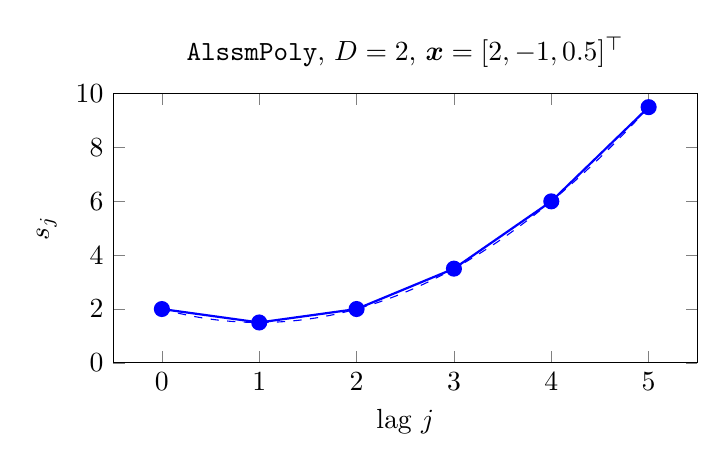
\begin{tikzpicture}
\begin{axis}[
  xlabel={lag $j$}, ylabel={$s_j$},
  title={\texttt{AlssmPoly}, $D=2$, $\vx=[2,-1,0.5]^\top$},
  xtick={0,1,2,3,4,5}, width=9cm, height=5cm,
  ymin=0, ymax=10,
  mark size=2.5pt
]
\addplot[blue, thick, mark=*, mark options={fill=blue}]
  coordinates {(0,2)(1,1.5)(2,2)(3,3.5)(4,6)(5,9.5)};
\addplot[blue, dashed, domain=0:5, samples=80]
  {2 - x + 0.5*x^2};
\end{axis}
\end{tikzpicture}
\end{center}

\subsection{State-transition matrix and output vector}

\begin{equation}
  \mA = \begin{bmatrix}
    1 & 1 & 1 \\
    0 & 1 & 2 \\
    0 & 0 & 1
  \end{bmatrix},
  \qquad
  \vC = [1,\; 0,\; 0].
\end{equation}
The $n$-th column of $\mA$ contains the binomial coefficients
$\binom{n}{k}$ for $k = 0, 1, \ldots, n$, so $\mA$ is the \emph{upper
Pascal matrix} of order $N = D+1$.

\subsection{Derivation of \texorpdfstring{$\mA$}{A}}

We must find $\mA$ such that $\mphi(j+1) = \mphi(j)\,\mA$ where
$\mphi(j) = [1,\, j,\, j^2,\, \ldots,\, j^D]$.  Column $n$ of $\mA$
must express $\phi_n(j+1) = (j+1)^n$ in terms of the basis evaluated
at $j$.  By the \textbf{binomial theorem}:
\begin{equation}
  (j+1)^n = \sum_{k=0}^{n} \binom{n}{k} j^k.
  \label{eq:binomial}
\end{equation}
Comparing with $\phi_n(j+1) = \sum_k A_{kn}\,\phi_k(j) = \sum_k A_{kn}\,
j^k$, we read off
\[
  A_{kn} = \binom{n}{k}, \quad 0 \leq k \leq n; \qquad A_{kn} = 0 \text{ for }
  k > n.
\]
This is precisely the \emph{upper Pascal matrix}:
\[
  \mA = \begin{bmatrix}
    \binom{0}{0} & \binom{1}{0} & \binom{2}{0} & \cdots \\
    0            & \binom{1}{1} & \binom{2}{1} & \cdots \\
    0            & 0            & \binom{2}{2} & \cdots \\
    \vdots       & \vdots       & \vdots       & \ddots
  \end{bmatrix}
  =
  \begin{bmatrix}
    1 & 1 & 1 & 1 & \cdots \\
    0 & 1 & 2 & 3 & \cdots \\
    0 & 0 & 1 & 3 & \cdots \\
    0 & 0 & 0 & 1 & \cdots \\
    \vdots & & & & \ddots
  \end{bmatrix}.
\]
The output vector $\vC = [1, 0, \ldots, 0]$ evaluates $s_0 = x_0$,
which is the polynomial value at the current sample ($j=0$).  This
follows from $\vC \mA^0 \vx = \vC \vx = x_0 = \vx|_{j=0}$.

\begin{remark}
The Pascal matrix is generated in lmlib via \texttt{scipy.linalg.pascal(N, kind='upper')}.
Its entries grow exponentially with degree and window size, causing the Gram
matrix $W = \sum_j \gamma^j \mphi(j)^\top \mphi(j)$ to have condition
number $\kappa(W) = \mathcal{O}(g^{2D})$ for effective window size $g$.
This is the main motivation for the alternative bases in the following
sections.
\end{remark}

% ============================================================
\section{\texttt{AlssmPolyJordan}: Falling-Factorial (Jordan) Basis}
\label{sec:jordan}
% ============================================================

\subsection{The polynomial family}

The Jordan basis replaces monomials $j^n$ with \emph{falling factorial}
polynomials (also called \emph{binomial coefficients in $j$}):
\begin{equation}
  \phi_n(j) \defeq \binom{j}{n} = \frac{j!}{n!\,(j-n)!}
           = \frac{j(j-1)\cdots(j-n+1)}{n!}, \quad
  \phi_0(j) = 1.
\end{equation}
The signal model is
\begin{equation}
  s_j(\vx) = \sum_{n=0}^{D} x_n \binom{j}{n}
           = x_0 + x_1 j + x_2 \frac{j(j-1)}{2} + \cdots
\end{equation}
Since $\binom{j}{n}$ is a degree-$n$ polynomial in $j$, this spans the
same function space as \texttt{AlssmPoly}.  The state coefficients
$x_n$ are the \emph{Newton forward-difference coefficients} of the signal
rather than the standard polynomial coefficients \cite{Zalmai2017}.

\subsection{Degree-2 example}

For $D=2$ the model is $s_j = x_0 + x_1 j + x_2 j(j-1)/2$.  With
$\vx = [2,\,-1,\,1]^\top$:
\begin{center}
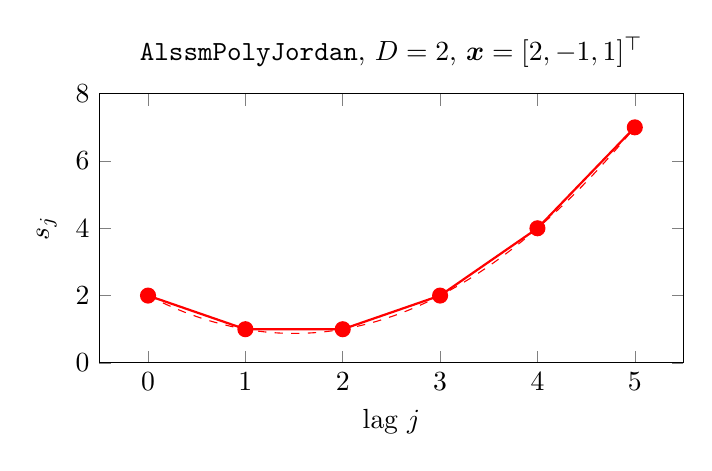
\begin{tikzpicture}
\begin{axis}[
  xlabel={lag $j$}, ylabel={$s_j$},
  title={\texttt{AlssmPolyJordan}, $D=2$, $\vx=[2,-1,1]^\top$},
  xtick={0,1,2,3,4,5}, width=9cm, height=5cm,
  ymin=0, ymax=8,
  mark size=2.5pt
]
\addplot[red, thick, mark=*, mark options={fill=red}]
  coordinates {(0,2)(1,1)(2,1)(3,2)(4,4)(5,7)};
\addplot[red, dashed, domain=0:5, samples=80]
  {2 - x + x*(x-1)/2};
\end{axis}
\end{tikzpicture}
\end{center}

\subsection{State-transition matrix and output vector}

\begin{equation}
  \mA = \begin{bmatrix}
    1 & 1 & 0 \\
    0 & 1 & 1 \\
    0 & 0 & 1
  \end{bmatrix},
  \qquad
  \vC = [1,\; 0,\; 0].
\end{equation}
This is the \emph{Jordan block} for eigenvalue $1$: the identity matrix
plus a superdiagonal of ones.  It is called the Jordan normal form because
it represents the nilpotent shift operator acting on a chain of generalised
eigenvectors \cite{Horn1985}.

\subsection{Derivation of \texorpdfstring{$\mA$}{A}}

We must verify that $\mphi(j+1) = \mphi(j)\,\mA$ with
$\mphi(j) = \bigl[\binom{j}{0}, \binom{j}{1}, \binom{j}{2}, \ldots\bigr]$.
This follows directly from \textbf{Pascal's identity}:
\begin{equation}
  \binom{j+1}{n} = \binom{j}{n} + \binom{j}{n-1}.
  \label{eq:pascal}
\end{equation}
Identifying $A_{kn}$ such that $\phi_n(j+1) = \sum_k A_{kn}\phi_k(j)$:
\[
  \binom{j+1}{n} = \binom{j}{n} + \binom{j}{n-1}
  \;\Longrightarrow\;
  A_{nn} = 1, \quad A_{n-1,n} = 1, \quad A_{kn} = 0 \text{ otherwise}.
\]
This gives the Jordan block $\mA = I + \mathrm{superdiag}(\mathbf{1})$.
The formula $A_{kn} = \delta_{k,n} + \delta_{k,n-1}$ creates the two
diagonals directly, without any free parameters.

\begin{remark}[Comparison with \texttt{AlssmPoly}]
Both bases span the same polynomial space. The Jordan basis has a far
simpler $\mA$ (bidiagonal vs.\ full upper triangular), and its condition
number $\kappa(\mA)$ grows more slowly with degree. However, both still
suffer from ill-conditioned Gram matrices for large windows, because the
design-matrix rows $\mphi(j)$ grow with $j$ in both bases. The Legendre
and Meixner bases address this directly.
\end{remark}

% ============================================================
\section{\texttt{AlssmPolyLegendre}: Legendre Basis on a Finite Window}
\label{sec:legendre}
% ============================================================

\subsection{Motivation}

For a finite window $[0, W]$, the monomial and falling-factorial design
matrices become ill-conditioned because $\phi_n(j) = j^n$ or
$\binom{j}{n}$ grow with $j$. The classical remedy is to \emph{normalise}
the lag index to a fixed interval and use an orthogonal polynomial basis.

\subsection{The polynomial family}

Let $W = b - a$ be the window width. Define the \emph{scaled lag}
\begin{equation}
  t_j \defeq \frac{2j}{W} - 1 \in [-1,+1], \qquad j \in [0, W],
  \label{eq:tsc}
\end{equation}
with step size $h = 2/W$.  The basis functions are the \emph{Legendre
polynomials} $P_n(t)$, which satisfy the three-term recurrence
\begin{equation}
  (n+1)P_{n+1}(t) = (2n+1)\,t\,P_n(t) - n\,P_{n-1}(t),
  \quad P_0(t)=1,\; P_1(t)=t.
  \label{eq:legendre3term}
\end{equation}
The signal model is
\begin{equation}
  s_j(\vx) = \sum_{n=0}^{D} x_n\, P_n(t_j).
\end{equation}
Key property: $\{P_n\}$ are orthogonal under the $L^2[-1,1]$ inner product,
\[
  \int_{-1}^{1} P_m(t)\,P_n(t)\,dt = \frac{2}{2n+1}\,\delta_{mn},
\]
which makes the continuous Gram matrix perfectly diagonal
\cite{Abramowitz1972, DLMF}.

\subsection{Degree-2 example ($W=10$, $h=0.2$)}

With $D=2$, $a_\text{seg}=0$, $b_\text{seg}=10$ the state
$\vx = [1,\, 0,\, 0]^\top$ gives the constant function $s_j = P_0(t_j) = 1$;
state $\vx = [0,\, 1,\, 0]^\top$ gives the ramp $s_j = t_j = h j - 1$; and
$\vx = [0,\, 0,\, 1]^\top$ gives the parabola $s_j = P_2(t_j) = (3t_j^2-1)/2$.

\begin{center}
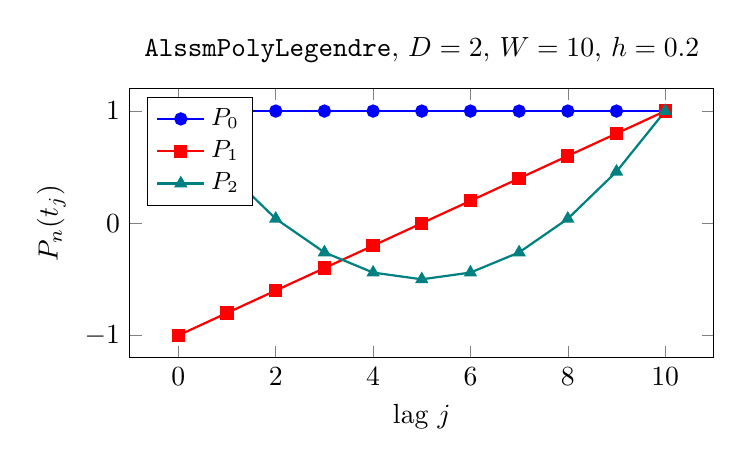
\begin{tikzpicture}
\begin{axis}[
  xlabel={lag $j$}, ylabel={$P_n(t_j)$},
  title={\texttt{AlssmPolyLegendre}, $D=2$, $W=10$, $h=0.2$},
  xtick={0,2,4,6,8,10},
  width=9cm, height=5cm,
  legend pos=north west,
  legend style={font=\small},
  mark size=2pt
]
\addplot[blue, thick, mark=*, mark options={fill=blue}]
  coordinates {(0,1)(1,1)(2,1)(3,1)(4,1)(5,1)(6,1)(7,1)(8,1)(9,1)(10,1)};
\addlegendentry{$P_0$}
\addplot[red, thick, mark=square*, mark options={fill=red}]
  coordinates {(0,-1)(1,-0.8)(2,-0.6)(3,-0.4)(4,-0.2)(5,0)(6,0.2)(7,0.4)(8,0.6)(9,0.8)(10,1)};
\addlegendentry{$P_1$}
\addplot[teal, thick, mark=triangle*, mark options={fill=teal}]
  coordinates {(0,1)(1,0.46)(2,0.04)(3,-0.26)(4,-0.44)(5,-0.5)(6,-0.44)(7,-0.26)(8,0.04)(9,0.46)(10,1)};
\addlegendentry{$P_2$}
\end{axis}
\end{tikzpicture}
\end{center}

\subsection{State-transition matrix and output vector}

For $D=2$, $W=10$ (i.e.\ $h=1/5$):
\begin{equation}
  \mA = \begin{bmatrix}
    1 & h & \tfrac{1}{2}h^2 + \tfrac{1}{6}h^2 \\[2pt]
    0 & 1 & 3h \\
    0 & 0 & 1
  \end{bmatrix}
  =
  \begin{bmatrix}
    1 & 0.2 & 0.06 \\
    0 & 1   & 0.6  \\
    0 & 0   & 1
  \end{bmatrix},
  \qquad
  \vC = \bigl[P_0(-1),\; P_1(-1),\; P_2(-1)\bigr] = [1,\; -1,\; 1].
\end{equation}
The matrix $\mA$ is upper-triangular with unit diagonal and is called the
\emph{Legendre shift matrix}; it has condition number $\kappa(\mA) \approx 1$
independently of $W$.

\subsection{Derivation of \texorpdfstring{$\mA$}{A}: Taylor shift in the Legendre basis}

The shift $j \to j+1$ corresponds to $t \to t + h$ in the scaled
coordinate.  We must express $P_n(t+h)$ as a linear combination of
$P_0(t), \ldots, P_n(t)$, i.e.\ find the column $n$ of $\mA$.

Expanding via the \textbf{Taylor series}:
\begin{equation}
  P_n(t+h) = \sum_{m=0}^{n} \frac{h^m}{m!}\, P_n^{(m)}(t),
  \label{eq:taylor}
\end{equation}
where $P_n^{(m)}$ is the $m$-th derivative.  Since $P_n^{(m)}$ is a
polynomial of degree $n-m$, it can be expanded in the Legendre basis:
\[
  P_n^{(m)}(t) = \sum_{k=0}^{n-m} \bigl[\mathbf{D}^m e_n\bigr]_k P_k(t),
\]
where $\mathbf{D}$ is the differentiation operator in Legendre coefficient
space (implemented by \texttt{numpy.polynomial.legendre.legder}), and
$e_n$ is the unit vector with a $1$ in position $n$.  Substituting:
\begin{equation}
  P_n(t+h) = \sum_{m=0}^{n} \frac{h^m}{m!}
             \sum_{k=0}^{n-m} \bigl[\mathbf{D}^m e_n\bigr]_k P_k(t).
\end{equation}
The coefficient of $P_k(t)$ in $P_n(t+h)$ is the $k$-th component of
\[
  A_{kn} = \sum_{m=0}^{n-k} \frac{h^m}{m!} \bigl[\mathbf{D}^m e_n\bigr]_k.
\]
This formula is \emph{exact} (not an approximation) because the Taylor
series of a polynomial terminates after finitely many terms.  It
requires only $O(N^2)$ operations and produces column $n$ of $\mA$
without any matrix inversion.

For $D=2$, $h=1/5$, the three columns work out as follows.
\begin{itemize}
  \item $n=0$: $P_0(t+h) = 1 = P_0(t)$, so column 0 = $[1,0,0]^\top$.
  \item $n=1$: $P_1(t+h) = t+h = P_1(t) + h\,P_0(t)$, so column 1 = $[h,1,0]^\top = [0.2,1,0]^\top$.
  \item $n=2$: $P_2(t+h) = \tfrac{3}{2}(t+h)^2 - \tfrac{1}{2}$
    $= \tfrac{3}{2}t^2 + 3th + \tfrac{3}{2}h^2 - \tfrac{1}{2}$
    $= P_2(t) + 3h\,P_1(t) + (\tfrac{3}{2}h^2 - \tfrac{1}{2} + \tfrac{1}{2})P_0(t)$
    $= P_2(t) + 3h\,P_1(t) + \tfrac{3}{2}h^2 P_0(t)$; noting
    $P_0(t) = 1$ and $\tfrac{3}{2}h^2 = \tfrac{3}{2} \cdot 0.04 = 0.06$,
    column 2 = $[0.06,\; 3h,\; 1]^\top = [0.06,\; 0.6,\; 1]^\top$.
\end{itemize}
This exactly matches the numerical $\mA$ above.

\begin{remark}[Output vector $\vC$]
The output vector evaluates the polynomial at the \emph{current} sample,
which has lag $j=0$ and thus scaled coordinate $t_0 = -1$.  Since
$P_n(-1) = (-1)^n$, the output vector is the alternating-sign vector
$\vC = [1, -1, 1, -1, \ldots]$.  When the segment window starts at
$a_\text{seg} \neq 0$, lmlib applies the additional shift
$\vC \leftarrow \vC\, \mA^{-a_\text{seg}}$ to keep the evaluation at
$j=0$.
\end{remark}

\begin{remark}[Gram-matrix conditioning]
The Gram matrix $W_{\rm ss} = V^\top \operatorname{diag}(\gamma^j) V$,
where $V_{jn} = P_n(t_j)$, has condition number
$\kappa(W_{\rm ss}) \approx 2D+1$ for all practical window sizes
\cite{Wildhaber2019}.  This is a reduction from $\kappa = \mathcal{O}(W^{2D})$
for the monomial basis.  The Legendre Vandermonde formula
$W_{\rm ss} = V^\top \operatorname{diag}(w)\,V$ is computed directly
without solving any linear system, giving exact results for any degree.
\end{remark}

% ============================================================
\section{\texttt{AlssmPolyMeixner}: Meixner Basis on a Semi-Infinite Window}
\label{sec:meixner}
% ============================================================

\subsection{Motivation}

\texttt{AlssmPolyLegendre} requires the window to be finite.  For
infinite or semi-infinite windows (as in the two-sided filter of
\texttt{ex122.0} or the baseline segments of \texttt{ex111.0}),
the window length is not a fixed integer but is controlled by the
exponential decay rate $\gamma = (g-1)/g$.  A basis that is
\emph{orthogonal under the geometric weight $\gamma^j$} on
$j = 0, 1, 2, \ldots$ is needed.

\subsection{The Meixner polynomial family}

The \emph{Meixner polynomials} $M_n(j;\, 1,\, \gamma)$ are the unique
(up to normalisation) family of polynomials satisfying
\begin{equation}
  \sum_{j=0}^{\infty} \gamma^j\, M_m(j)\, M_n(j)
  = \frac{\delta_{mn}}{(1-\gamma)\,\gamma^n}
  \label{eq:meixner_orthog}
\end{equation}
for all $m, n \geq 0$, where $0 < \gamma < 1$ \cite{Koekoek1996, DLMF}.
They are given explicitly by the hypergeometric series
\begin{equation}
  M_n(j;\, 1,\, \gamma) = {}_2F_1\!\left(-n,\, -j;\, 1;\, 1-\tfrac{1}{\gamma}\right)
  = \sum_{k=0}^{\min(n,j)} (-1)^k \binom{n}{k}\binom{j}{k}\left(1-\tfrac{1}{\gamma}\right)^{\!k},
  \label{eq:meixner_explicit}
\end{equation}
where ${}_2F_1$ is the Gauss hypergeometric function.

Two special values are essential:
\begin{align}
  M_n(0;\, 1,\, \gamma) &= 1 \quad\text{for all }n \geq 0,
    \label{eq:meixner_at_zero}\\[4pt]
  \sum_{j=0}^{\infty} \gamma^j\,\bigl[M_n(j;\,1,\gamma)\bigr]^2
    &= \frac{1}{(1-\gamma)\,\gamma^n} \quad\text{for all }n \geq 0.
    \label{eq:meixner_norm}
\end{align}
Equation~\eqref{eq:meixner_at_zero} follows because setting $j=0$ kills every
term in~\eqref{eq:meixner_explicit} except $k=0$, giving
$(-1)^0\binom{n}{0}\binom{0}{0}(1-1/\gamma)^0=1$.
Equation~\eqref{eq:meixner_norm} is the squared $\ell^2_\gamma$-norm of $M_n$:
it equals the diagonal entry $W_{\rm ss}[n,n]$ of the steady-state Gram
matrix, and follows from~\eqref{eq:meixner_orthog} with $m=n$.

\subsection{Degree-2 example ($g=5$, $\gamma=4/5$)}

The first three Meixner polynomials for $\gamma = 4/5$
evaluate as follows ($h = 1-1/\gamma = -1/4$):
\[
  M_0(j) = 1, \quad M_1(j) = 1 + jh = 1 - \tfrac{j}{4}, \quad
  M_2(j) = 1 + 2jh + j(j-1)h^2 / \text{something}\ldots
\]
Numerically: $M_1(0)=1$, $M_1(1)=0.75$, $M_1(2)=0.5$, $M_1(3)=0.25$,
$M_1(4)=0$, $M_1(5)=-0.25$; and
$M_2(0)=1$, $M_2(1)=0.5$, $M_2(2)=0.0625$, $M_2(3)=-0.3125$,
$M_2(4)=-0.625$.

\begin{center}
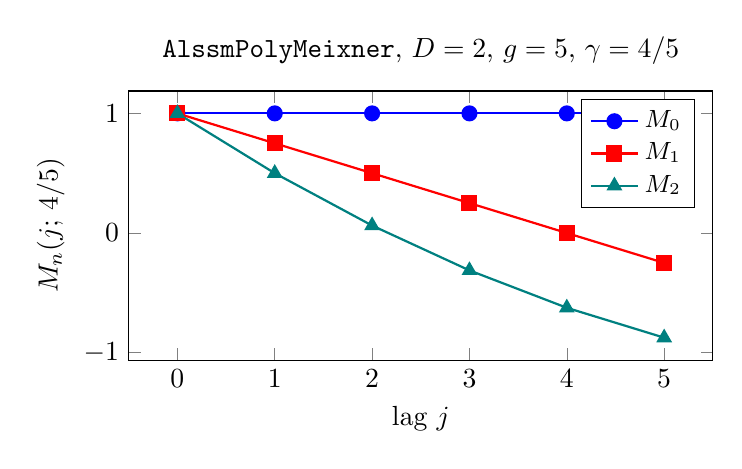
\begin{tikzpicture}
\begin{axis}[
  xlabel={lag $j$}, ylabel={$M_n(j;\,4/5)$},
  title={\texttt{AlssmPolyMeixner}, $D=2$, $g=5$, $\gamma=4/5$},
  xtick={0,1,2,3,4,5},
  width=9cm, height=5cm,
  legend pos=north east,
  legend style={font=\small},
  mark size=2.5pt
]
\addplot[blue, thick, mark=*, mark options={fill=blue}]
  coordinates {(0,1)(1,1)(2,1)(3,1)(4,1)(5,1)};
\addlegendentry{$M_0$}
\addplot[red, thick, mark=square*, mark options={fill=red}]
  coordinates {(0,1)(1,0.75)(2,0.5)(3,0.25)(4,0)(5,-0.25)};
\addlegendentry{$M_1$}
\addplot[teal, thick, mark=triangle*, mark options={fill=teal}]
  coordinates {(0,1)(1,0.5)(2,0.0625)(3,-0.3125)(4,-0.625)(5,-0.875)};
\addlegendentry{$M_2$}
\end{axis}
\end{tikzpicture}
\end{center}

\subsection{State-transition matrix and output vector}

For general $g$ (and $\gamma = (g-1)/g$, $D \geq 1$):
\begin{equation}
  \mA = I_N - \frac{1}{g-1}\,\triu(\mathbf{1}_N,\, 1)
  =
  \begin{bmatrix}
    1 & -\tfrac{1}{g-1} & -\tfrac{1}{g-1} & \cdots \\
    0 & 1               & -\tfrac{1}{g-1} & \cdots \\
    0 & 0               & 1               & \cdots \\
    \vdots & & & \ddots
  \end{bmatrix},
  \qquad
  \vC = [1,\; 1,\; \ldots,\; 1].
  \label{eq:meixner_A}
\end{equation}
For $g=5$ ($\gamma=4/5$), $D=2$:
\begin{equation}
  \mA = \begin{bmatrix}
    1 & -0.25 & -0.25 \\
    0 & 1     & -0.25 \\
    0 & 0     & 1
  \end{bmatrix}, \qquad \vC = [1,\; 1,\; 1].
\end{equation}
The output vector $\vC = \mathbf{1}^\top$ follows from~\eqref{eq:meixner_at_zero}:
evaluating at $j=0$ gives $s_0 = \sum_n x_n M_n(0) = \sum_n x_n$.

\subsection{Derivation of \texorpdfstring{$\mA$}{A}}

We must find $\mA$ such that
$\mphi(j+1) = \mphi(j)\,\mA$ where $\mphi(j) = [M_0(j), M_1(j), \ldots, M_D(j)]$.
Column $n$ of $\mA$ must express $M_n(j+1)$ as a linear combination of
$M_0(j), \ldots, M_D(j)$.

\medskip
\noindent\textbf{Step 1: Forward difference from the explicit formula.}
Starting from~\eqref{eq:meixner_explicit} we compute the first-order
forward difference $\Delta[M_n](j) \defeq M_n(j+1) - M_n(j)$:
\[
  \Delta[M_n](j)
  = \sum_{k=0}^{n} (-1)^k\binom{n}{k}\!\left(1-\tfrac{1}{\gamma}\right)^k
    \!\bigl[\binom{j+1}{k} - \binom{j}{k}\bigr].
\]
By \textbf{Pascal's identity} $\binom{j+1}{k} - \binom{j}{k} = \binom{j}{k-1}$,
so the $k=0$ term vanishes and we shift $k \to k+1$:
\begin{equation}
  \Delta[M_n](j)
  = -\!\left(1-\tfrac{1}{\gamma}\right)\!
    \sum_{k=0}^{n-1} (-1)^k\binom{n}{k+1}\!\left(1-\tfrac{1}{\gamma}\right)^k
    \binom{j}{k}.
  \label{eq:diff1}
\end{equation}

\medskip
\noindent\textbf{Step 2: Express as partial sum of Meixner polynomials.}
From~\eqref{eq:meixner_explicit}, the $k$-th term of $M_m(j)$ is
$(-1)^k\binom{m}{k}(1-1/\gamma)^k\binom{j}{k}$.
Summing over $m = 0, 1, \ldots, n-1$:
\[
  \sum_{m=0}^{n-1} M_m(j)
  = \sum_{k=0}^{n-1} (-1)^k\!\left(1-\tfrac{1}{\gamma}\right)^k\binom{j}{k}
    \underbrace{\sum_{m=k}^{n-1}\binom{m}{k}}_{= \binom{n}{k+1}},
\]
where the inner sum is evaluated by the \textbf{hockey-stick identity}
\cite{Graham1994}:
\begin{equation}
  \sum_{m=k}^{n-1}\binom{m}{k} = \binom{n}{k+1}.
  \label{eq:hockeystick}
\end{equation}
Comparing with~\eqref{eq:diff1} and noting that
$-(1-1/\gamma) = 1/g - 1 = (1-g)/g$; since $1-1/\gamma = -1/g$ (for $\gamma = (g-1)/g$):
\begin{equation}
  \Delta[M_n](j) = M_n(j+1) - M_n(j)
  = -\frac{1-\gamma}{\gamma} \sum_{m=0}^{n-1} M_m(j)
  = -\frac{1}{g-1} \sum_{m=0}^{n-1} M_m(j),
  \label{eq:meixner_shift_identity}
\end{equation}
using $(1-\gamma)/\gamma = 1/(g-1)$.

\medskip
\noindent\textbf{Step 3: Read off $\mA$.}
Rearranging~\eqref{eq:meixner_shift_identity}:
\[
  M_n(j+1) = M_n(j) - \frac{1}{g-1}\sum_{m=0}^{n-1}M_m(j)
  = \sum_{k=0}^{D} A_{kn}\, M_k(j),
\]
with
\[
  A_{kn} =
  \begin{cases}
    1           & k = n, \\
    -\dfrac{1}{g-1} & k < n, \\
    0           & k > n.
  \end{cases}
\]
This is precisely $\mA = I_N - \tfrac{1}{g-1}\,\triu(\mathbf{1}_N, 1)$, confirming~\eqref{eq:meixner_A}.

\begin{remark}[Gram-matrix conditioning]
From the orthogonality relation~\eqref{eq:meixner_orthog}, the steady-state
Gram matrix $W_{\rm ss}$ is diagonal with entries
\begin{equation}
  W_{\rm ss}[n,n] = \frac{\gamma^{-\delta}}{(1-\gamma)\,\gamma^n}
                  = g \left(\frac{g}{g-1}\right)^{\!n},
\end{equation}
giving condition number
\[
  \kappa(W_{\rm ss}) = \left(\frac{g}{g-1}\right)^{\!D},
\]
which grows only algebraically (and very slowly) with degree $D$.
For $g=20$, $D=5$: $\kappa \approx 1.29$.  Compare to $\kappa = \mathcal{O}(g^{2D}) \approx 10^{19}$
for the monomial basis \cite{Wildhaber2019}.
\end{remark}

\begin{remark}[Comparison with Legendre]
While both Legendre and Meixner achieve near-unity Gram-matrix condition numbers,
they are complementary:
\begin{itemize}
  \item \textbf{Legendre}: for \emph{finite} windows; the Legendre polynomials
    are orthogonal under the \emph{uniform} weight on $\{0,\ldots,W\}$.
    Meixner is not orthogonal on finite windows (the orthogonality requires
    the infinite tail of the geometric sum to converge).
  \item \textbf{Meixner}: for \emph{semi-infinite} or \emph{bi-infinite}
    exponential windows; the Meixner polynomials are orthogonal under the
    \emph{geometric} weight $\gamma^j$ on $\{0,1,2,\ldots\}$.
    For finite windows with moderate $g$, Legendre has lower $\kappa(W_{\rm ss})$.
\end{itemize}
The crossover occurs around $W \approx 8g$: for $W < 8g$, Legendre is better
conditioned; for $W > 8g$, Meixner is.
\end{remark}

\begin{remark}[Xi-recursion drift]
The $\xi$-recursion in lmlib accumulates $\xi[k] = \xi[k-1] + \ldots$ over
$K$ time steps.  Rounding errors grow proportionally to $\kappa(\mA)^K$.
For \texttt{AlssmPoly} with large $g$, $\kappa(\mA) = \mathcal{O}(g^D)$,
causing catastrophic drift at degree $D \geq 13$ (for $g=20$, observed in
testing).  For \texttt{AlssmPolyMeixner},
$\kappa(\mA) \approx 1 + D/(g-1) \leq 2$ for all $D \leq g-1$, so the
recursion remains stable through at least $D=24$ (the limit of numerical
tests performed).  \texttt{AlssmPolyLegendre} has the same drift behaviour
as \texttt{AlssmPolyMeixner} for finite windows, both being stable through
$D \approx 20$ with catastrophic divergence appearing around $D \geq 22$.
\end{remark}

% ============================================================
\section{Comparison and Selection Guide}
% ============================================================

\begin{table}[h]
\centering
\caption{Comparison of polynomial ALSSM bases. $D$: polynomial degree;
$W$: window width; $g$: effective window size.}
\label{tab:comparison}
\renewcommand{\arraystretch}{1.4}
\begin{tabular}{lcccc}
\toprule
Property & \texttt{Poly} & \texttt{Jordan} & \texttt{Legendre} & \texttt{Meixner} \\
\midrule
$\kappa(\mA)$                & $\mathcal{O}(g^D)$    & $\mathcal{O}(D^2)$    & $\approx 1$          & $\approx 1 + D/(g-1)$ \\
$\kappa(W_{\rm ss})$         & $\mathcal{O}(W^{2D})$ & $\mathcal{O}(W^{2D})$ & $\approx 2D+1$       & $(g/(g-1))^D$         \\
$W_{\rm ss}$ fast path       & Stein solver          & Stein solver          & Vandermonde          & Diagonal (exact)       \\
Valid window type            & any                   & any                   & finite               & $\infty$ / semi-$\infty$ \\
Max. stable degree (approx.) & 12                    & $\sim 15$             & 21                   & $>24$                  \\
State $\vx$ interpretation   & monomial coeffs       & Newton coeffs         & Legendre coeffs      & Meixner coeffs         \\
\bottomrule
\end{tabular}
\end{table}

\smallskip
\noindent$^\dagger$\,\textit{Drift-free degree}: the highest polynomial
degree at which the $\xi$-recursion does not exhibit catastrophic numerical
drift over $K=50\,000$ samples on a constant signal ($y\equiv 1$), measured
as $\operatorname{std}(\hat{y}) < 10^{-3}$ in the steady-state window.
Drift originates from rounding-error accumulation proportional
to $\kappa(\mA)^K$ and limits the usable degree of \texttt{AlssmPoly} and
\texttt{AlssmPolyJordan} far more severely than Gram-matrix conditioning alone.

\bigskip
\smallskip
\noindent$^\dagger$\,\textit{Drift-free degree}: highest polynomial degree
at which the $\xi$-recursion does not exhibit catastrophic numerical drift
over $K=50\,000$ samples on a constant signal ($y\equiv 1$), measured as
$\operatorname{std}(\hat{y})<10^{-3}$ in the steady-state portion of the signal.
Drift arises from floating-point error accumulation proportional to
$\kappa(\mA)^K$, and limits the usable degree of \texttt{AlssmPoly} and
\texttt{AlssmPolyJordan} far more severely than Gram-matrix conditioning.

\bigskip
\noindent\textbf{Practical selection rules:}
\begin{itemize}
  \item For finite windows with large $g$ (near-rectangular): use
    \texttt{AlssmPolyLegendre}.
  \item For semi-infinite or bi-infinite windows: use
    \texttt{AlssmPolyMeixner} with $g$ set to the effective window size of
    the dominant segment.
  \item For multi-segment composite costs with both finite and infinite
    segments: use \texttt{AlssmPolyMeixner} tuned to the infinite segment's $g$.
  \item For $D \leq 3$ and any window: all four classes are numerically
    equivalent; prefer \texttt{AlssmPoly} for simplicity and interpretability.
\end{itemize}

% ============================================================
\section*{References}
% ============================================================

\begingroup
\renewcommand{\section}[2]{}
\begin{thebibliography}{99}

\bibitem{Wildhaber2018}
R.\ Wildhaber, H.\ Loeliger, and F.\ Waldmann,
``Polynomial smoothing filters and recursive Legendre differentiation,''
\emph{IEEE Transactions on Signal Processing}, vol.\ 66, no.\ 5, pp.\ 1108--1123, 2018.
DOI: \href{https://doi.org/10.1109/TSP.2017.2787124}{10.1109/TSP.2017.2787124}

\bibitem{Wildhaber2019}
R.\ Wildhaber,
\emph{Nonparametric Signal Analysis with Autonomous Linear State Space Models},
Ph.D.\ Thesis, ETH Zürich, 2019.
\href{https://www.research-collection.ethz.ch/handle/20.500.11850/357916}{ETH Research Collection}

\bibitem{Zalmai2017}
N.\ Zalmai,
\emph{Causal and Non-Causal Signal Analysis with ALSSM},
Ph.D.\ Thesis, ETH Zürich, 2017.
\href{https://www.research-collection.ethz.ch/handle/20.500.11850/176652}{ETH Research Collection}

\bibitem{Koekoek1996}
R.\ Koekoek and R.\ F.\ Swarttouw,
``The Askey-scheme of hypergeometric orthogonal polynomials and its
$q$-analogue,''
Technical Report 94-05, Delft University of Technology, 1996.
\href{https://arxiv.org/abs/math/9602214}{arXiv:math/9602214}

\bibitem{DLMF}
NIST Digital Library of Mathematical Functions,
Chapter 18: Orthogonal Polynomials.
\url{https://dlmf.nist.gov/18}

\bibitem{Abramowitz1972}
M.\ Abramowitz and I.\ A.\ Stegun,
\emph{Handbook of Mathematical Functions}, 10th~ed.\
Dover, New York, 1972.

\bibitem{Graham1994}
R.\ L.\ Graham, D.\ E.\ Knuth, and O.\ Patashnik,
\emph{Concrete Mathematics: A Foundation for Computer Science}, 2nd~ed.\
Addison-Wesley, 1994.

\bibitem{Horn1985}
R.\ A.\ Horn and C.\ R.\ Johnson,
\emph{Matrix Analysis}.
Cambridge University Press, 1985.

\end{thebibliography}
\endgroup

\end{document}
